\chapter{序論}
\label{chap_intro}

\section{研究背景}
従来の内視鏡の生検は食道,大腸,小腸,胃などを鉗子で2 mm角程度の立方体で抜き出し,染色したものを2,3断面にカットしてから病理診断医が顕微鏡で観察し,腫瘍か非腫瘍かを判別したり,その悪性度を判定している.断面のみの観察では内部に腫瘍がある場合に見落としてしまうリスクがある
そこで組織透明化技術(LUCID-A)\cite{sekitani2016ultraflexible}を用いて内視鏡検体を透明化して丸ごと観察する.

\begin{figure}[H]
	\centering
	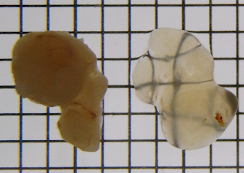
\includegraphics[width=0.7\linewidth]{fig/chapter1/lucid}
	\caption{Transparent specimen}
	\label{fig:lucid}
\end{figure}

がん検診では見落としなく病変を見つけることが求められているため,担当医が判定してから専門医がダブルチェックをしている.現在の日本の病理の専門医は2483名\cite{pathology}で,その人数に対して標本500万件を年間で処理している現状である.現在でも専門医の負担は大きいと言えるが,透明化技術で全断面を観察可能となれば,全てを専門医が診断することは現実的ではない.
そこで,人工知能がスクリーニングを行って専門医の確認が必要な症例を絞り込んで診断することが求められる.

\section{先行研究}
人工知能に関する研究は現在盛んに行われ,特に画像認識の分野では深層学習\cite{lecun2015deep}を利用した研究チームがILSVRC2012という画像認識の大会でこれまでは少しの改良を続けてきたところを,深層学習を利用することで一気に画像認識の精度を高めるという衝撃があり,その後は深層学習を用いたモデル同士で画像認識を競うようになった.今では95\%以上の認識率を超えて,人間よりも高い認識精度を達成している.

この画像認識の技術を医療画像でも利用する研究が行われている.深層学習を用いた医療画像の診断アルゴリズムの先行研究としては,乳がん\cite{wang2016deep}の検体や皮膚がん\cite{esteva2017dermatologist}などがある.これらの検体の認識では深層学習を利用して専門医と同程度の精度を達成している.
しかしこのような精度を出すためには,数万枚の画像データを用意する必要があることに加えて,その画像を認識する目的のカテゴリーに分類する作業(アノテーション)が必要がある.
少量の画像データしか用意できないと,様々なバリエーションに対応することができないという問題や,深層学習の訓練に用いるデータが医師によってばらつきがある場合は教師データを作成した医師の判断が大きく反映されてしまうという問題が生じる.これらの課題があるため医療画像における深層学習を用いた診断システムは,大量にデータを用意するまでの時間や人的コストを大きく払うことになっているのが現状である.

3次元画像を解析する先行研究としては,CTやMRI画像が上げられる\cite{dou20163d}.CTやMRIの場合は,画像の分解能が顕微鏡像よりも低く,深さ方向にも1ステップ数mmオーダーで30枚程度であるため,2次元画像の深層学習による解析を3次元にそのまま拡張して解析することができ,見落としを防止する診断のアルゴリズムを作ることができている.しかし本研究のように深さ方向に数百ステップある画像を解析することは深層学習の訓練に使うパラメータが大きくなり過ぎて学習が安定しないという問題がある.

\section{本研究の目的}
本研究の目的は,内視鏡生検を透明にして深層学習を利用して癌を見落とさない診断方法を開発することである.組織透明化技術LUCIDを用いて検体を丸ごと透明化し,共焦点レーザー顕微鏡で観察することで検体の内部まで3次元情報として解析することができる.

\begin{figure}[H]
	\centering
	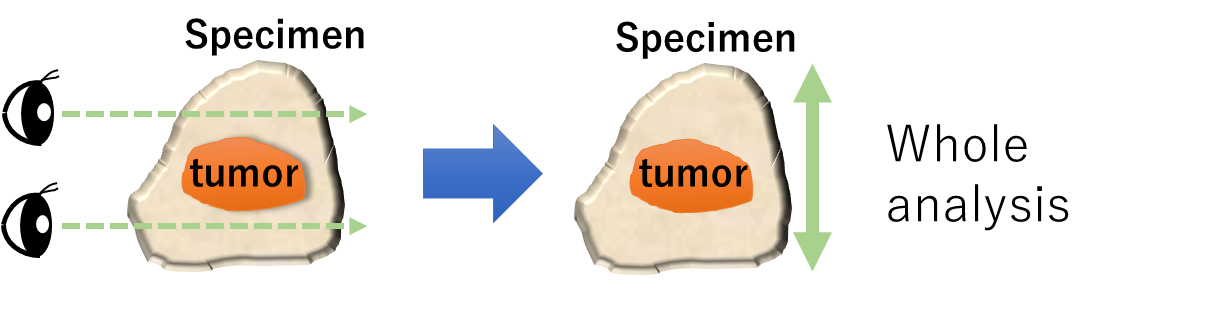
\includegraphics[width=0.8\linewidth]{fig/chapter1/whole_image_analysis}
	\caption{Schematic of whole image analysis}
	\label{fig:wholeimageanalysis}
\end{figure}

透明化されたサンプルを共焦点レーザー顕微鏡で撮影すると,従来のカットする手法に換算して1000断面に相当する.そのため,得られる顕微鏡撮影像が従来の2,3カットに対して数100倍となるので,専門医が診断をする負担が大きくなってしまう.そこで,人工知能(Artificial Intelligence: AI)が3次元画像を解析して病変を検知し,専門医に提示することで病変の見落としリスク(偽陰性)がゼロになる診断支援システムを開発することが本研究の目的である.

生検検体の3次元画像を解析することで2次元画像では判断の難しいものを3次元特有の情報を用いることで判定精度を上げる.本研究で用いる透明化処理した検体は共焦点レーザー顕微鏡で撮影するため分解能が高く,深さ方向にも1ステップ数$\upmu$mオーダーで400〜700枚が撮影することができる.このように深さ方向にも分解能が高い3次元画像でも特徴を抽出できるように解析する手法を研究する.

深層学習で解析を行う場合はデータを大量に準備する必要がある.今回のように,新しい撮影手法であったり,希少な病気であったりすると医療データを数多く集められないことがある.さらに画像データだけでなく,その画像に教師ラベルを貼る(アノテーションをする)必要がある.画像とその教師ラベルのセットを数万枚と集めることができれば,高い精度で腫瘍を検出できるという報告があるが\cite{esteva2017dermatologist},少ない教師データで識別精度を上げることは深層学習において困難とされている.

画像の構造的な特徴のパターンを学ぶ教師なし学習と呼ばれる手法では教師ラベルを必要とせず画像データがあれば良い.これの教師なり学習と教師ラベルを使った学習を組み合わせた,半教師あり学習(弱教師あり学習)によって病理画像が正常から異常になる過程には連続的な性質があることを活用して正常と異常の分布を学習し,より正常と腫瘍の認識精度を高める.

最後にこの深層学習による腫瘍の検出結果を医師が診断する際のサポートになるように可視化することに取り組んだ.深層学習は判断の理由が分からないためブラックボックスと呼ばれ,信頼性が求められる場面では利用に対して不安視されることがある.そのため腫瘍と正常の診断の判断の理由を可視化する必要がある.
明らかに正常のものと,腫瘍かもしれない領域で区別して,腫瘍かもしれない部分を医師に提示することで腫瘍を見落とさないような医師の負担を減らすためのスクリーニングとして利用するため可視化処理を行う.

\begin{figure}[H]
	\centering
	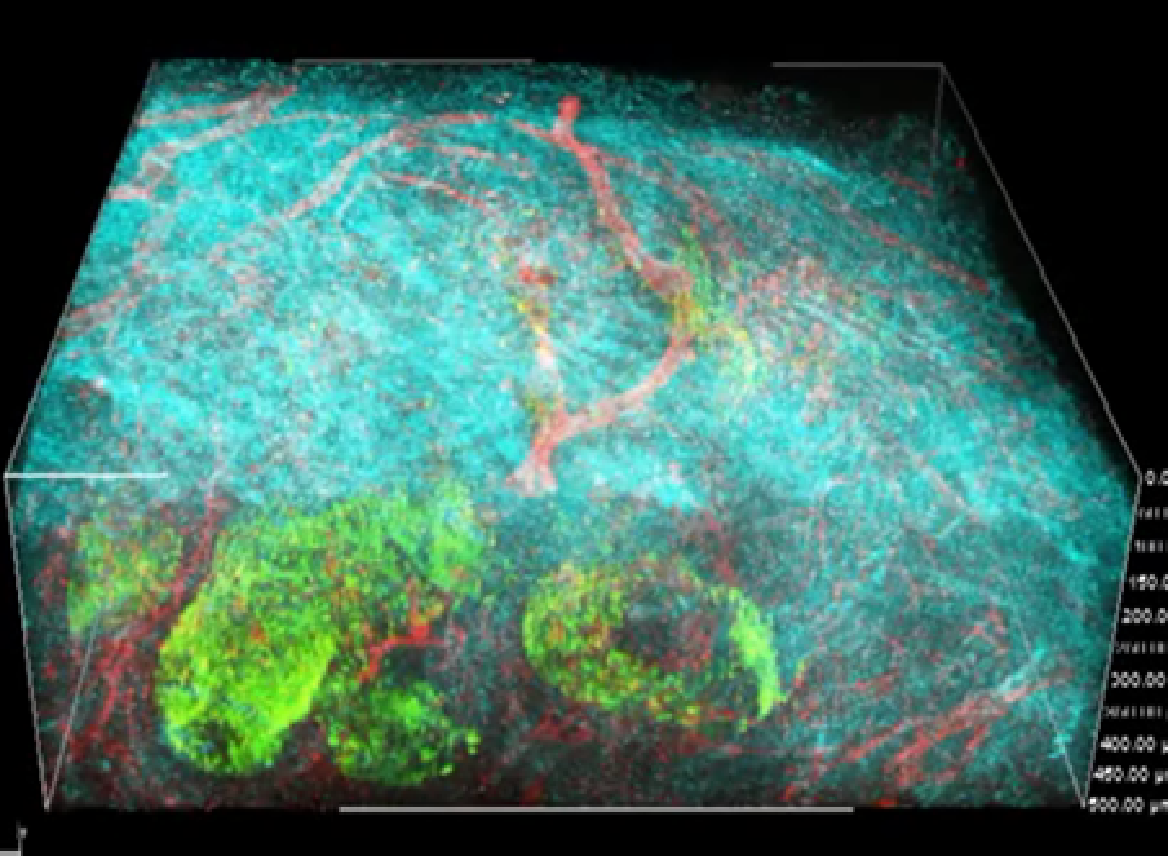
\includegraphics[width=0.7\linewidth]{fig/chapter1/microscope}
	\caption{Image taken by multi focus laser microscope}
	\label{fig:microscope}
\end{figure}
